\documentclass[12pt]{fphw}

\usepackage[utf8]{inputenc}
\usepackage[T1]{fontenc}
\usepackage{mathpazo}
\usepackage{alphabeta}
\usepackage{graphicx}
\usepackage{booktabs}
\usepackage{listings}
\usepackage{enumerate}
\usepackage{hyperref}
\usepackage{amsmath}
\usepackage{framed}
\usepackage[framed]{ntheorem}
\usepackage{amssymb}
\usepackage{xcolor}
\usepackage{tabularx}
\usepackage{tikz}
\usepackage{float}
\usepackage{array}

\graphicspath{{./figures/}}

\newframedtheorem{frm-thm}{Theorem}
\hypersetup{
    colorlinks=true,
    linkcolor=blue,
    filecolor=magenta,
    urlcolor=cyan,
}
\urlstyle{same}

\title{Deep Learning for NLP}
\author{Αλέξανδρος Γκιάφης \\ID: sdi2200284}
\date{Spring Semester 2025-2026}
\institute{National and Kapodistrian University of Athens \\ Department of Informatics and Telecommunications}
\class{Artificial Intelligence II (YS19 Μ226 Μ262 Μ325 Μ405)}

\begin{document}
\maketitle

{
  \hypersetup{linkcolor=black}
  \tableofcontents
}
\newpage

\section{Abstract}

Σκοπός της εργασίας ήταν να κατασκευαστεί ένα μοντέλο που, για ένα ζεύγος ερώτησης--απάντησης, προβλέπει αν η απάντηση είναι \emph{Clear Reply}, \emph{Ambivalent} ή \emph{Clear Non-Reply}. Δηλαδή δεν αρκεί να δούμε αν η απάντηση έχει λέξεις σχετικές με την ερώτηση. Πρέπει να καταλάβουμε αν ο ομιλητής όντως απαντάει, αν αποφεύγει την απάντηση, ή αν βρίσκεται κάπου ενδιάμεσα. Αυτό κάνει το πρόβλημα αρκετά δύσκολο, ειδικά επειδή πολλές πολιτικές απαντήσεις περιέχουν πληροφορία αλλά ταυτόχρονα έχουν και υπεκφυγή.

Η τελική μου προσέγγιση βασίστηκε σε pretrained Transformer μοντέλα, κυρίως στο DeBERTa-v3-base \cite{he2021deberta}. Δοκίμασα πρώτα DistilBERT \cite{sanh2019distilbert} και BERT \cite{devlin2019bert}, ώστε να έχω μικρότερα και μεγαλύτερα σημεία αναφοράς. Στη συνέχεια χρησιμοποίησα DeBERTa, επειδή είχε καθαρά καλύτερη απόδοση στο validation set. Πάνω στο DeBERTa πρόσθεσα προσεκτικά feature engineering από την πρώτη εργασία, όχι όμως βάζοντας τεχνητά tokens μέσα στο κείμενο, αλλά ως ξεχωριστά αριθμητικά χαρακτηριστικά σε ένα μικρό neural head.

Το καλύτερο public Kaggle αποτέλεσμα που πέτυχα ήταν 0.69 macro-F1, που αντιστοιχούσε στην 31η θέση στο public leaderboard. Στο validation set η καλύτερη τοπική εκδοχή έφτασε 0.7136 macro-F1 με ensemble από τρεις διαφορετικές όψεις του ίδιου DeBERTa μοντέλου. Το public leaderboard μπορεί να μην είναι απόλυτα ίδιο με το private leaderboard, αλλά μου έδωσε μια ρεαλιστική εικόνα της γενίκευσης.

\section{Data processing and analysis}

\subsection{Pre-processing}

Το αρχικό training set είχε 3448 γραμμές. Πριν την εκπαίδευση έκανα καθαρισμό και έμειναν 3412 παραδείγματα. Ο καθαρισμός είχε δύο βασικά βήματα. Πρώτον, αφαιρέθηκαν διπλότυπα ζεύγη ερώτησης--απάντησης που είχαν αντικρουόμενες ετικέτες. Αν το ίδιο ακριβώς ζεύγος εμφανίζεται με δύο διαφορετικά labels, τότε το μοντέλο λαμβάνει αντιφατικό σήμα. Δεύτερον, αφαιρέθηκαν μερικές προβληματικές γραμμές που είχαν εντοπιστεί από την ανάλυση OOV της πρώτης εργασίας.

Δεν έκανα υπερβολικό καθάρισμα του φυσικού κειμένου, γιατί τα Transformer μοντέλα είναι ήδη προεκπαιδευμένα πάνω σε πραγματικό, ακατέργαστο κείμενο. Αν αφαιρούσα πολλά σημεία στίξης, αριθμούς ή μικρές φράσεις, υπήρχε κίνδυνος να πετάξω χρήσιμη πληροφορία. Για παράδειγμα, μια απάντηση που ξεκινά με ``well'', ``I think'', ή ``let me be clear'' μπορεί να δείχνει ύφος υπεκφυγής ή προσπάθεια ευθυγράμμισης με την ερώτηση. Αυτά τα σήματα δεν ήθελα να τα καταστρέψω.

Δοκίμασα όμως και μία πιο ελεγχόμενη κανονικοποίηση λέξεων. Η ιδέα ήταν ότι σε αυτή την εργασία δεν μας ενδιαφέρει απαραίτητα ο ακριβής αριθμός, π.χ. το 1981, αλλά το ότι υπάρχει μια χρονιά. Έτσι, σε ένα πείραμα αντικατέστησα μοτίβα όπως χρονιές, χρήματα, ποσοστά και ημερομηνίες με κανονικές αγγλικές λέξεις όπως \texttt{year}, \texttt{money}, \texttt{percent}. Αυτό είναι διαφορετικό από το να βάλουμε άγνωστα tokens όπως \texttt{[A\_YEAR]}. Με πραγματικές λέξεις, το DeBERTa έχει ήδη κάποιο νόημα από την προεκπαίδευσή του. Με τεχνητά tokens, πρέπει να μάθει καινούρια embeddings από περίπου 3000 παραδείγματα, κάτι που αποδείχθηκε πολύ αδύναμο.

\subsection{Analysis}

Οι τρεις κλάσεις δεν είναι το ίδιο εύκολες. Η \emph{Ambivalent} κλάση είναι η πιο ύπουλη, επειδή βρίσκεται ανάμεσα στις άλλες δύο. Μια απάντηση μπορεί να δίνει κάποια πληροφορία αλλά όχι πλήρη απάντηση. Αυτό σημαίνει ότι το μοντέλο πρέπει να μάθει λεπτές διαφορές, όχι απλώς λέξεις-κλειδιά.

Από την ανάλυση λαθών φάνηκε ότι τα περισσότερα δύσκολα παραδείγματα είναι μεγάλες πολιτικές απαντήσεις. Συχνά έχουν πολλά στοιχεία, αιτιολογήσεις, αβεβαιότητα και αλλαγή θέματος. Για παράδειγμα, το μοντέλο πολλές φορές προέβλεπε \emph{Ambivalent} με μεγάλη σιγουριά ενώ η σωστή κλάση ήταν \emph{Clear Reply} ή \emph{Clear Non-Reply}. Αυτό δείχνει ότι η μεσαία κλάση λειτουργεί σαν ``μαγνήτης'' για αβέβαιες περιπτώσεις.

Στο καλύτερο DeBERTa single model με numeric features, ο confusion matrix ήταν:
\[
\begin{bmatrix}
69 & 34 & 2 \\
34 & 155 & 13 \\
1 & 9 & 25
\end{bmatrix}
\]
όπου οι γραμμές είναι οι πραγματικές κλάσεις και οι στήλες οι προβλέψεις. Το βασικό πρόβλημα είναι ότι πολλά \emph{Clear Reply} και αρκετά \emph{Clear Non-Reply} πηγαίνουν στο \emph{Ambivalent}. Αυτό είναι λογικό για το συγκεκριμένο task: όταν το μοντέλο δεν είναι σίγουρο αν η απάντηση είναι καθαρή ή υπεκφυγή, επιλέγει τη μεσαία κατηγορία.

\subsection{Data partitioning for train, test and validation}

Χώρισα τα καθαρισμένα δεδομένα σε train και validation με αναλογία 90/10 και stratification ως προς την κλάση. Συγκεκριμένα, χρησιμοποίησα 3070 παραδείγματα για εκπαίδευση και 342 για validation. Το stratification ήταν σημαντικό, επειδή το macro-F1 επηρεάζεται πολύ από τις μικρότερες κλάσεις. Αν το validation set είχε τυχαία πολύ λίγα παραδείγματα από μία κλάση, το score θα ήταν πολύ θορυβώδες.

Δεν έκανα μεγάλο cross-validation, κυρίως λόγω χρόνου και GPU κόστους. Αντί για αυτό, έτρεξα αρκετές ελεγχόμενες δοκιμές με ίδιο split, ώστε κάθε αλλαγή να συγκρίνεται όσο γίνεται δίκαια με την προηγούμενη. Σε μερικές κρίσιμες φάσεις δοκίμασα και διαφορετικά seeds, επειδή στα Transformer fine-tuning πειράματα το seed μπορεί να αλλάξει αρκετά το αποτέλεσμα.

\subsection{Vectorization}

Στα κλασικά μοντέλα η αναπαράσταση του κειμένου έγινε με TF-IDF. Αυτό σημαίνει ότι κάθε κείμενο μετατρέπεται σε ένα μεγάλο sparse διάνυσμα, όπου κάθε διάσταση αντιστοιχεί σε μια λέξη ή n-gram και η τιμή δείχνει πόσο σημαντικός είναι αυτός ο όρος στο συγκεκριμένο κείμενο. Αυτό είναι δυνατό baseline, αλλά δεν καταλαβαίνει καλά σειρά λέξεων, ειρωνεία, ή σύνθετη σχέση ερώτησης--απάντησης.

Στα Transformer μοντέλα η vectorization γίνεται διαφορετικά. Ο tokenizer χωρίζει την ερώτηση και την απάντηση σε subword tokens. Μετά το pretrained μοντέλο παράγει contextual embeddings, δηλαδή διανύσματα που εξαρτώνται από τα συμφραζόμενα. Για παράδειγμα, η λέξη ``clear'' δεν έχει πάντα το ίδιο διάνυσμα· το διάνυσμά της αλλάζει ανάλογα με τις γύρω λέξεις. Αυτό είναι ο βασικός λόγος που BERT/DeBERTa είναι πιο κατάλληλα για το πρόβλημα από ένα απλό bag-of-words μοντέλο.

Η είσοδος δινόταν ως ζεύγος: ερώτηση ως πρώτο sequence και απάντηση ως δεύτερο sequence. Έτσι το μοντέλο μπορούσε να συγκρίνει την απάντηση με την ερώτηση, αντί να ταξινομεί μόνο την απάντηση απομονωμένα.

\section{Algorithms and Experiments}

\subsection{Experiments}

Ξεκίνησα από απλούστερα μοντέλα και σταδιακά πήγα σε πιο δυνατές προσεγγίσεις. Αυτό ήταν χρήσιμο γιατί κάθε επίπεδο έδινε ένα σημείο αναφοράς. Αν ένα πιο περίπλοκο μοντέλο δεν κερδίζει το απλό, τότε μάλλον κάτι πάει λάθος.

Το αρχικό baseline από την πρώτη εργασία ήταν Logistic Regression με TF-IDF και είχε περίπου 0.6017 macro-F1 στο validation. Αυτό είναι αξιοπρεπές για κλασικό μοντέλο, αλλά η εργασία απαιτούσε deep learning προσέγγιση και το leaderboard έδειχνε ότι τα καλύτερα αποτελέσματα ήταν αρκετά υψηλότερα.

Μετά δοκίμασα DistilBERT. Το DistilBERT είναι μια μικρότερη και ταχύτερη εκδοχή του BERT. Δεν είναι απλώς ``μικρό BERT'', αλλά μοντέλο που έχει εκπαιδευτεί ώστε να μιμείται μεγαλύτερο μοντέλο με λιγότερες παραμέτρους. Το καλύτερο DistilBERT έφτασε 0.6405 macro-F1 με \texttt{max\_length=512}. Αυτό έδειξε ότι το μεγαλύτερο context βοηθάει σε ένα μικρότερο μοντέλο, επειδή πολλές απαντήσεις είναι μεγάλες.

Στη συνέχεια δοκίμασα BERT-base. Το BERT-base είναι μεγαλύτερο από το DistilBERT και χρησιμοποιεί bidirectional self-attention, δηλαδή όταν αναπαριστά μια λέξη κοιτάει και αριστερά και δεξιά στο κείμενο. Το καλύτερο BERT έφτασε 0.6417 macro-F1, πολύ κοντά στο DistilBERT. Αυτό μου έδειξε ότι το απλό BERT δεν ήταν αρκετό breakthrough από μόνο του.

Το μεγάλο άλμα ήρθε με DeBERTa-v3-base. Το DeBERTa είναι Transformer σαν το BERT, αλλά αλλάζει τον τρόπο που χειρίζεται τη θέση και το περιεχόμενο των tokens. Με απλά λόγια, προσπαθεί να ξεχωρίσει καλύτερα το ``τι λέει μια λέξη'' από το ``πού βρίσκεται μέσα στην πρόταση''. Αυτό μπορεί να βοηθήσει σε ερωτήσεις--απαντήσεις όπου η σειρά και η δομή της απάντησης παίζουν ρόλο. Το DeBERTa single model έφτασε 0.6962 macro-F1, πολύ καλύτερα από DistilBERT/BERT.

Στην πορεία δοκίμασα αρκετές ιδέες που δεν δούλεψαν. Μία ήταν να βάλω τεχνητά feature tokens μέσα στο κείμενο, όπως tags για hedge, overlap ή μήκος απάντησης. Αυτό απέτυχε γιατί το DeBERTa δεν ξέρει από πριν τι σημαίνουν αυτά τα tokens. Έπρεπε να τα μάθει από λίγα δεδομένα, και τελικά το validation έπεσε περίπου στο 0.61. Το μάθημα ήταν ότι το feature engineering της πρώτης εργασίας δεν πρέπει να μπει βίαια μέσα στο κείμενο.

Η πιο χρήσιμη ιδέα ήταν να κρατήσω το κείμενο καθαρό και να βάλω τα handcrafted features ως αριθμητικά χαρακτηριστικά. Δηλαδή το DeBERTa διαβάζει κανονικά την ερώτηση και την απάντηση, και παράλληλα ένα μικρό MLP διαβάζει features όπως μήκος απάντησης, overlap ερώτησης--απάντησης, δείκτες αβεβαιότητας και δομικά χαρακτηριστικά. Στο τέλος ενώνω το embedding του DeBERTa με το embedding των features και κάνω την τελική ταξινόμηση. Αυτό έδωσε το καλύτερο submitted αποτέλεσμα.

Δοκίμασα επίσης evasion labels. Η ιδέα ήταν ότι, αφού το dataset έχει πιο λεπτομερή ετικέτα υπεκφυγής στο train, ίσως ένα δεύτερο μοντέλο να προβλέπει πιθανότητες evasion και αυτές να βοηθούν την clarity ταξινόμηση. Το έκανα με out-of-fold προβλέψεις ώστε να μην υπάρχει leakage. Παρόλα αυτά, το score έπεσε στο 0.6503. Η πιθανή εξήγηση είναι ότι το evasion taxonomy είναι συγγενικό αλλά όχι ίδιο με το clarity label. Το μοντέλο μπερδεύτηκε από λεπτές κατηγορίες υπεκφυγής που δεν αντιστοιχούν καθαρά στις τρεις τελικές κλάσεις.

Τέλος, δοκίμασα focused answer views και dual-view architecture. Το focused view κρατούσε την αρχή της απάντησης, προτάσεις με overlap με την ερώτηση και το τέλος. Η ιδέα ήταν να μειωθεί ο θόρυβος στις τεράστιες απαντήσεις. Μόνο του δεν κέρδισε, επειδή πολλές φορές η συνολική ρητορική ροή της απάντησης είναι σημαντική. Όμως ως μέρος ensemble βοήθησε λίγο, επειδή έκανε διαφορετικά λάθη από το full answer μοντέλο. Το dual-view μοντέλο, όπου περνούσα full και focused input από DeBERTa και ένωνα τα δύο outputs, ήταν πιο πολύπλοκο και τελικά υπερεκπαιδεύτηκε.

\subsubsection{Table of trials}

\begin{table}[H]
\centering
\small
\begin{tabularx}{\textwidth}{lXrr}
\toprule
Trial & Περιγραφή & Val macro-F1 & Public Kaggle \\
\midrule
HW1 baseline & Logistic Regression με TF-IDF & 0.6017 & -- \\
DistilBERT & \texttt{max\_length=512}, lr $3e^{-5}$, 3 epochs & 0.6405 & -- \\
BERT & \texttt{max\_length=256}, lr $2e^{-5}$, 5 epochs & 0.6417 & -- \\
DeBERTa & απλό two-segment input, 3 epochs & 0.6962 & περίπου 0.68 \\
DeBERTa ensemble & weighted ensemble από seeds & 0.7070 & 0.68 \\
Feature tokens & handcrafted tags μέσα στο κείμενο & 0.6191 & δεν υποβλήθηκε \\
Numeric features & DeBERTa + αριθμητικό side branch & 0.7057 & \textbf{0.69} \\
More epochs & ίδια ιδέα με 6 epochs & 0.6958 & 0.67 \\
Rich features & πολλά επιπλέον HW1-style features & 0.6593 & 0.64 \\
Evasion stack & πιθανότητες evasion ως extra features & 0.6503 & δεν υποβλήθηκε \\
Word normalization & αντικατάσταση αριθμών με κανονικές λέξεις & 0.7084 & -- \\
Focused ensemble & raw + wordnorm + focused view & \textbf{0.7136} & -- \\
Dual-view & full και focused είσοδος μαζί & 0.6888 & δεν υποβλήθηκε \\
\bottomrule
\end{tabularx}
\caption{Κύρια πειράματα. Το public Kaggle score που κρατήθηκε ως τελικό ήταν 0.69, 31η θέση.}
\label{tab:trials}
\end{table}

\subsection{Hyper-parameter tuning}

Τα βασικά hyperparameters που ρύθμισα ήταν learning rate, αριθμός epochs, \texttt{max\_length}, weight decay και seed. Για DistilBERT το \texttt{max\_length=512} βοήθησε, επειδή το μοντέλο χρειαζόταν περισσότερη απάντηση για να αποφασίσει. Για DeBERTa όμως το \texttt{max\_length=512} δεν βοήθησε. Έπεσε στο 0.6615, πιθανότατα επειδή το batch size έπρεπε να μικρύνει και η εκπαίδευση έγινε πιο θορυβώδης.

Το DeBERTa ήταν επίσης ευαίσθητο στο seed. Για παράδειγμα, στο numeric feature setup το seed 42 έφτασε 0.7007, ενώ τα seeds 0 και 1 ήταν 0.6462 και 0.6684. Για αυτό δεν εμπιστεύτηκα τυφλά ένα μόνο seed. Έκανα weighted ensembles, αλλά όχι απλό μέσο όρο όταν κάποια seeds ήταν πολύ χειρότερα. Το καλύτερο Phase 12 ensemble έδωσε βάρη 0.9 στο seed 42, 0.0 στο seed 0 και 0.1 στο seed 1.

Δοκίμασα περισσότερα epochs, επειδή υπήρχε υποψία ότι το μοντέλο δεν είχε μάθει αρκετά. Αυτό δεν επιβεβαιώθηκε. Στα 6 epochs το validation και το Kaggle score έπεσαν. Άρα το πρόβλημα δεν ήταν underfitting αλλά overfitting ή αλλαγή της training trajectory. Με λίγα δεδομένα, ένα δυνατό Transformer μπορεί να αρχίσει γρήγορα να προσαρμόζεται υπερβολικά στο train split.

\subsection{Optimization techniques}

Χρησιμοποίησα AdamW optimizer \cite{loshchilov2019adamw}, που είναι η συνηθισμένη επιλογή για fine-tuning Transformer μοντέλων. Σε DeBERTa χρειάστηκε ειδική προσοχή, γιατί αρχικά το training έβγαζε NaN ή κατέρρεε προβλέποντας σχεδόν μόνο \emph{Ambivalent}. Το διόρθωσα με σταθερή έκδοση \texttt{transformers==4.44.0}, \texttt{eps=1e-6} στον optimizer και διαφορετικό learning rate για backbone και classifier head. Το head έπαιρνε μεγαλύτερο learning rate, ώστε να προσαρμοστεί πιο γρήγορα στις τρεις κλάσεις.

Στα numeric-feature μοντέλα τα αριθμητικά features κανονικοποιήθηκαν με βάση μόνο το train split. Αυτό είναι σημαντικό για να μην περάσει πληροφορία από το validation ή το test set στο training. Μετά πέρασαν από μικρό MLP και ενώθηκαν με το pooled representation του DeBERTa. Με αυτόν τον τρόπο το μοντέλο μπορούσε να συνδυάσει semantic πληροφορία από το κείμενο με ρητά σήματα όπως μήκος, overlap και ύφος.

Για τα ensembles δεν επανεκπαίδευσα νέο μοντέλο. Κράτησα τις πιθανότητες των επιμέρους μοντέλων και έκανα alpha sweep στο validation set. Δηλαδή δοκίμασα διαφορετικά βάρη στον μέσο όρο πιθανοτήτων και διάλεξα αυτά που μεγιστοποιούσαν το macro-F1.

\subsection{Evaluation}

Η βασική μετρική ήταν macro-F1. Το F1 για μία κλάση είναι ο αρμονικός μέσος precision και recall:
\[
F1 = 2 \cdot \frac{precision \cdot recall}{precision + recall}
\]
Το macro-F1 υπολογίζει το F1 κάθε κλάσης ξεχωριστά και μετά παίρνει τον μέσο όρο. Αυτό είναι σωστό για το task, επειδή δεν θέλουμε το μοντέλο να είναι καλό μόνο στην πιο συχνή κλάση. Αν ένα μοντέλο προβλέπει συνέχεια \emph{Ambivalent}, μπορεί να έχει ανεκτό accuracy, αλλά θα έχει κακό macro-F1 επειδή αγνοεί τις άλλες κλάσεις.

\subsubsection{ROC curve}

\begin{figure}[H]
\centering
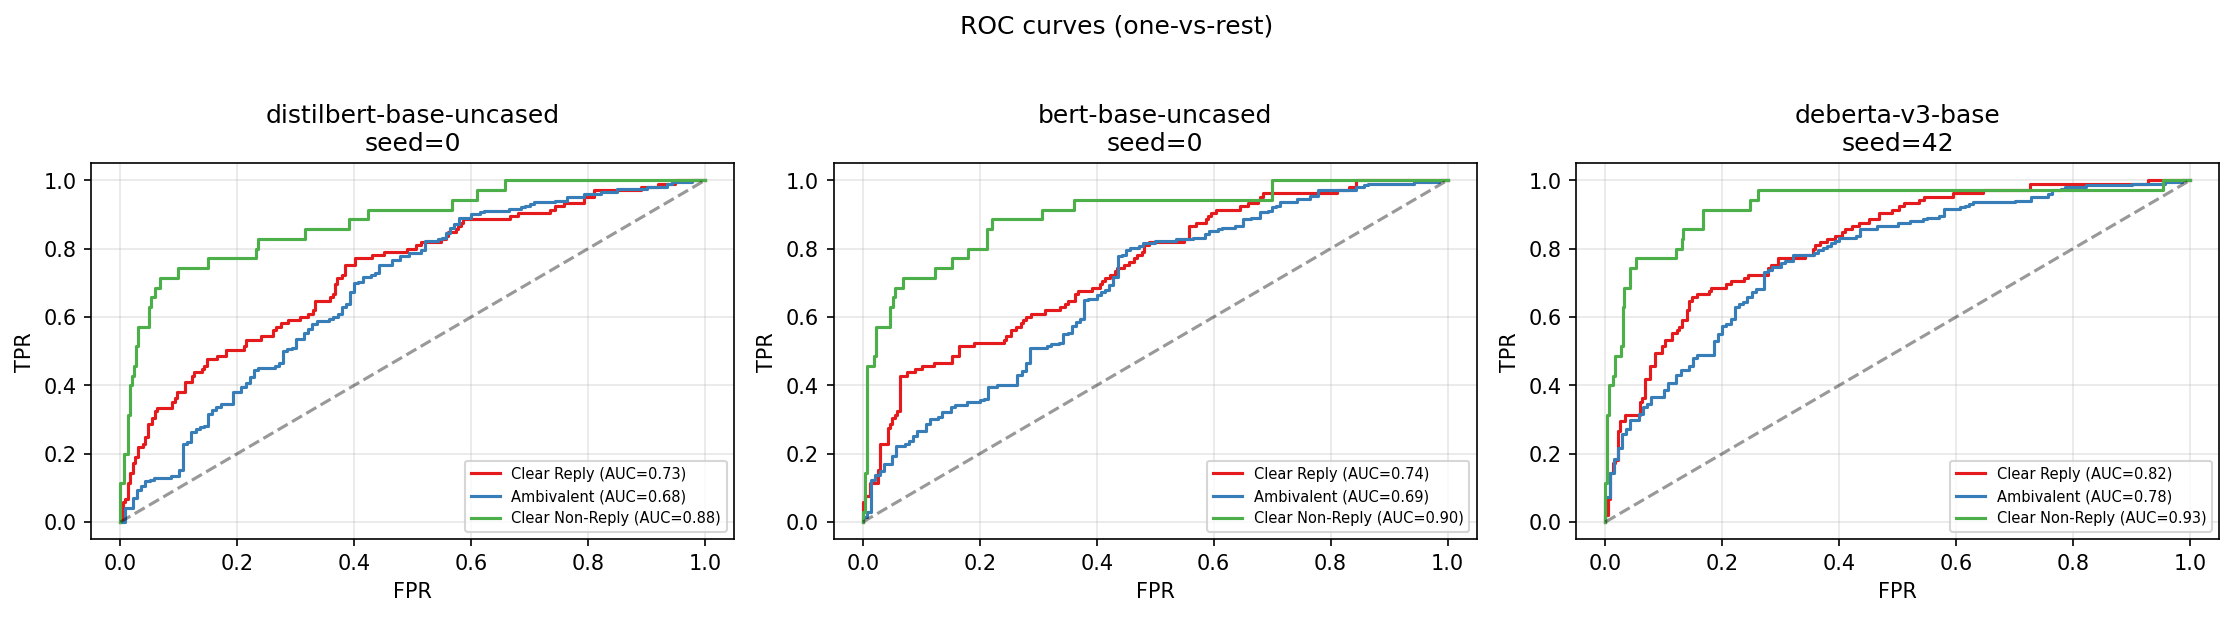
\includegraphics[width=0.92\textwidth]{roc_curves.png}
\caption{ROC curves για τα βασικά μοντέλα. Οι καμπύλες βοηθούν να δούμε πόσο καλά διαχωρίζει κάθε μοντέλο τις κλάσεις σε διαφορετικά thresholds.}
\label{fig:roc}
\end{figure}

\subsubsection{Learning Curve}

\begin{figure}[H]
\centering
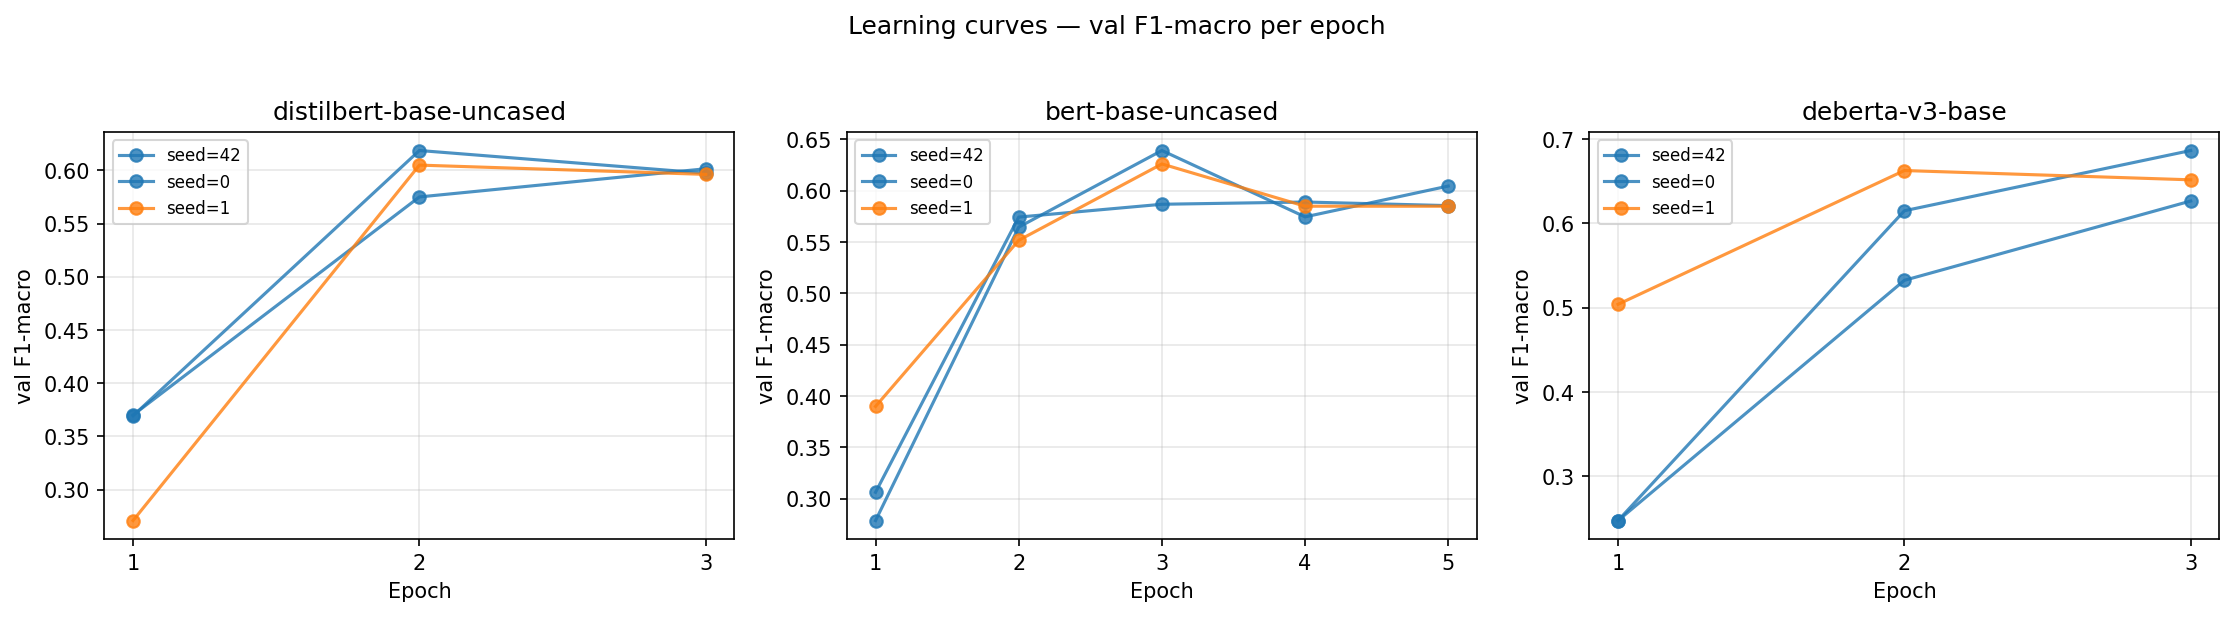
\includegraphics[width=0.92\textwidth]{learning_curves.png}
\caption{Learning curves. Στα πιο δυνατά μοντέλα φαίνεται ότι μετά από λίγα epochs το validation δεν βελτιώνεται σταθερά, ένδειξη ότι το dataset είναι μικρό για πολύ επιθετικό fine-tuning.}
\label{fig:learning}
\end{figure}

\subsubsection{Confusion matrix}

\begin{figure}[H]
\centering
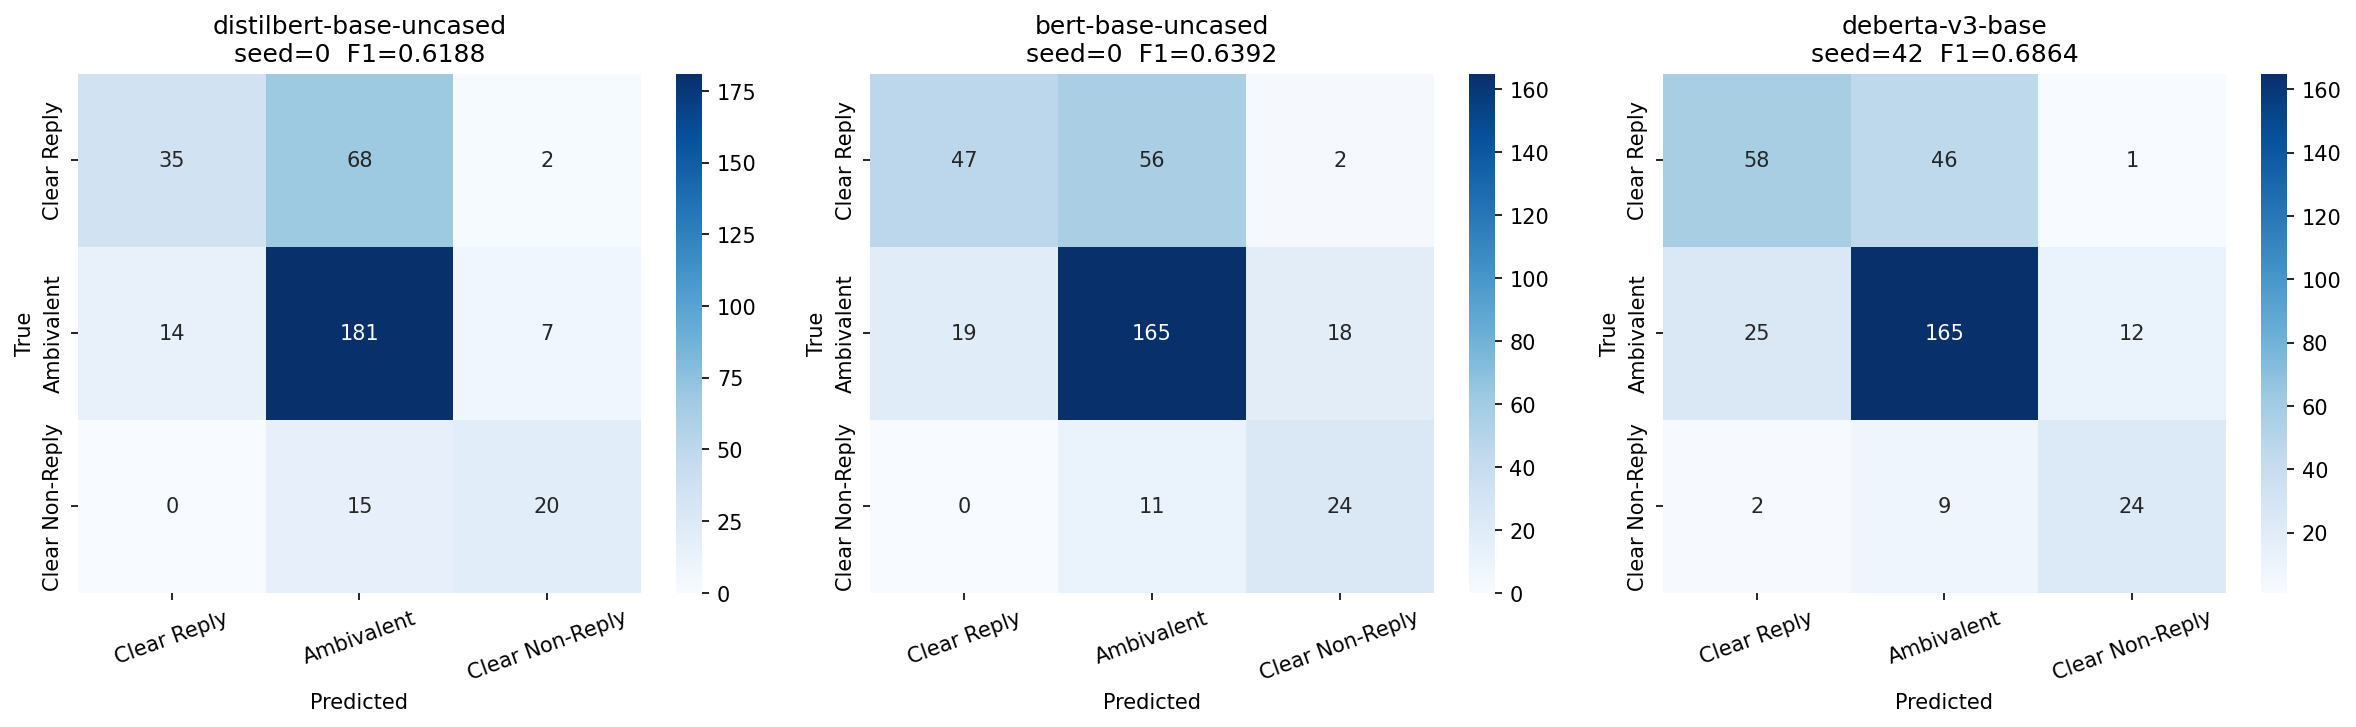
\includegraphics[width=0.92\textwidth]{confusion_matrices.png}
\caption{Confusion matrices των βασικών runs. Το πιο συχνό μοτίβο λάθους είναι η μετακίνηση καθαρών απαντήσεων ή μη-απαντήσεων προς την ενδιάμεση Ambivalent κλάση.}
\label{fig:confusion}
\end{figure}

\begin{figure}[H]
\centering
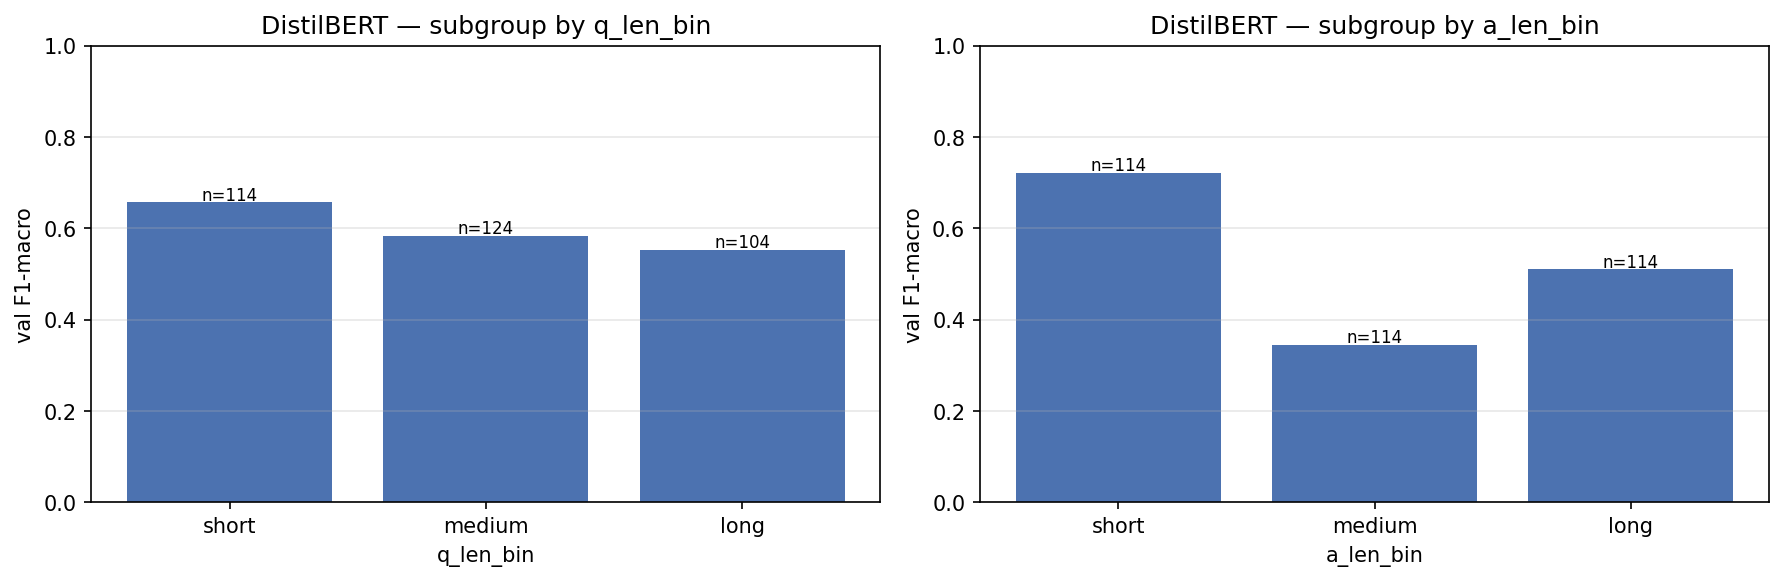
\includegraphics[width=0.92\textwidth]{subgroup_analysis.png}
\caption{Subgroup analysis. Τα λάθη αυξάνονται σε μεγάλες απαντήσεις και σε απαντήσεις με αβεβαιότητα, αιτιολογήσεις ή αριθμητικές λεπτομέρειες.}
\label{fig:subgroups}
\end{figure}

\section{Results and Overall Analysis}

\subsection{Results Analysis}

Το τελικό αποτέλεσμα είναι καλό σε σχέση με τα αρχικά baselines, αλλά όχι τέλειο σε σχέση με την κορυφή του leaderboard. Από περίπου 0.60 macro-F1 με TF-IDF φτάσαμε 0.69 public Kaggle και πάνω από 0.71 local validation σε ensemble. Αυτό δείχνει ότι τα pretrained Transformer μοντέλα όντως έμαθαν καλύτερη σχέση ερώτησης--απάντησης.

Παρόλα αυτά, η εργασία έδειξε και τα όρια του απλού ``βάζω περισσότερα features''. Στην πρώτη εργασία πολλά handcrafted features βοηθούσαν, επειδή το linear μοντέλο δεν είχε τρόπο να καταλάβει μόνο του overlap, hedge words ή δομή. Στο DeBERTa όμως πολλά από αυτά τα σήματα υπάρχουν ήδη έμμεσα μέσα στα embeddings. Όταν πρόσθεσα πάρα πολλά features, το μοντέλο χειροτέρεψε. Αυτό δεν σημαίνει ότι το feature engineering είναι άχρηστο. Σημαίνει ότι πρέπει να μπει με τρόπο που συμπληρώνει το pretrained μοντέλο και όχι με τρόπο που το μπερδεύει.

Το πιο χαρακτηριστικό παράδειγμα ήταν η διαφορά ανάμεσα σε feature tokens και numeric side branch. Τα feature tokens ήταν κακή ιδέα, επειδή ζητούσαν από το DeBERTa να μάθει άγνωστα σύμβολα. Το numeric side branch ήταν καλύτερη ιδέα, επειδή άφηνε το κείμενο φυσικό και πρόσθετε τα features ξεχωριστά.

Η ανάλυση λαθών έδειξε ότι το πρόβλημα δεν είναι απλώς lexical coverage. Πολλές λανθασμένες απαντήσεις περιέχουν λέξεις της ερώτησης και αρκετές πληροφορίες, αλλά η τελική τους στάση είναι ασαφής. Αυτό εξηγεί γιατί τα coverage/evidence features και το focused cropping δεν έδωσαν breakthrough. Για να αποφασίσεις αν μια πολιτική απάντηση είναι καθαρή, συχνά χρειάζεσαι ολόκληρη τη ρητορική πορεία της απάντησης, όχι μόνο τις προτάσεις με overlap.

\subsubsection{Best trial}

Το καλύτερο submitted trial ήταν το DeBERTa με numeric features και weighted ensemble. Η αρχιτεκτονική ήταν:

\begin{enumerate}
    \item Το DeBERTa-v3-base λαμβάνει την ερώτηση και την απάντηση ως two-segment input.
    \item Υπολογίζονται αριθμητικά features από το ζεύγος ερώτησης--απάντησης.
    \item Τα features κανονικοποιούνται με statistics από το train split.
    \item Ένα μικρό MLP μετατρέπει τα features σε dense representation.
    \item Το representation του DeBERTa και το representation των features ενώνονται.
    \item Ένας classifier προβλέπει τις τρεις clarity κλάσεις.
\end{enumerate}

Το καλύτερο single run αυτής της οικογένειας είχε 0.7007 validation macro-F1. Το weighted ensemble έφτασε 0.7057 validation macro-F1 και πέτυχε 0.69 στο public Kaggle leaderboard, 31η θέση. Η πιο πρόσφατη τοπική εκδοχή, Phase 18, είχε ακόμα καλύτερο validation score 0.7136, συνδυάζοντας raw full answer, word-normalized full answer και focused raw answer. Δεν την αναφέρω ως public αποτέλεσμα, επειδή το αξιόπιστο leaderboard score που κρατήθηκε ως τελικό είναι το 0.69.

\subsection{Comparison with the first project}

Σε σχέση με την πρώτη εργασία, η βασική διαφορά είναι ότι τώρα το μοντέλο δεν βασίζεται μόνο σε χειροποίητα χαρακτηριστικά και TF-IDF. Στην πρώτη εργασία το feature engineering ήταν ο κύριος τρόπος να δώσω στο μοντέλο γνώση για το πρόβλημα. Για παράδειγμα, αν ήθελα να ξέρει ότι μια απάντηση είναι μεγάλη, έπρεπε να του δώσω explicit feature. Αν ήθελα να ξέρει overlap με την ερώτηση, έπρεπε να το υπολογίσω εγώ.

Στα Transformer μοντέλα, μεγάλο μέρος αυτής της πληροφορίας μαθαίνεται από το ίδιο το pretrained μοντέλο. Το DeBERTa έχει ήδη μάθει πολλές γλωσσικές σχέσεις από τεράστια corpora πριν δει το δικό μας dataset. Έτσι μπορεί να καταλάβει καλύτερα παραφράσεις, ύφος και συμφραζόμενα. Αυτό εξηγεί γιατί το DeBERTa ξεπέρασε καθαρά το HW1 baseline.

Όμως η πρώτη εργασία δεν ήταν άχρηστη. Αντίθετα, η τελική βελτίωση ήρθε όταν πήρα την ιδέα του feature engineering από εκεί και την πρόσθεσα πιο προσεκτικά στο neural μοντέλο. Το καλύτερο αποτέλεσμα δεν ήταν ούτε καθαρό DeBERTa ούτε καθαρό feature engineering, αλλά συνδυασμός: DeBERTa για semantic κατανόηση και λίγα αριθμητικά features για explicit σήματα που το μοντέλο μπορεί να μη χρησιμοποιεί σταθερά.

Αν είχα περισσότερο χρόνο, θα δοκίμαζα πιο συστηματικό ablation των features, περισσότερα seeds για το Phase 18 ensemble και πιθανώς calibration πάνω σε μεγαλύτερο validation set. Θα ήμουν πιο προσεκτικός με πολύπλοκες αρχιτεκτονικές όπως dual-view, γιατί με μόνο περίπου 3000 training examples το μοντέλο έχει μεγάλη πιθανότητα να υπερεκπαιδευτεί.

\section{Bibliography}

\bibliographystyle{plain}
\bibliography{refs}

\end{document}
